\begin{figure*}
  \centering
  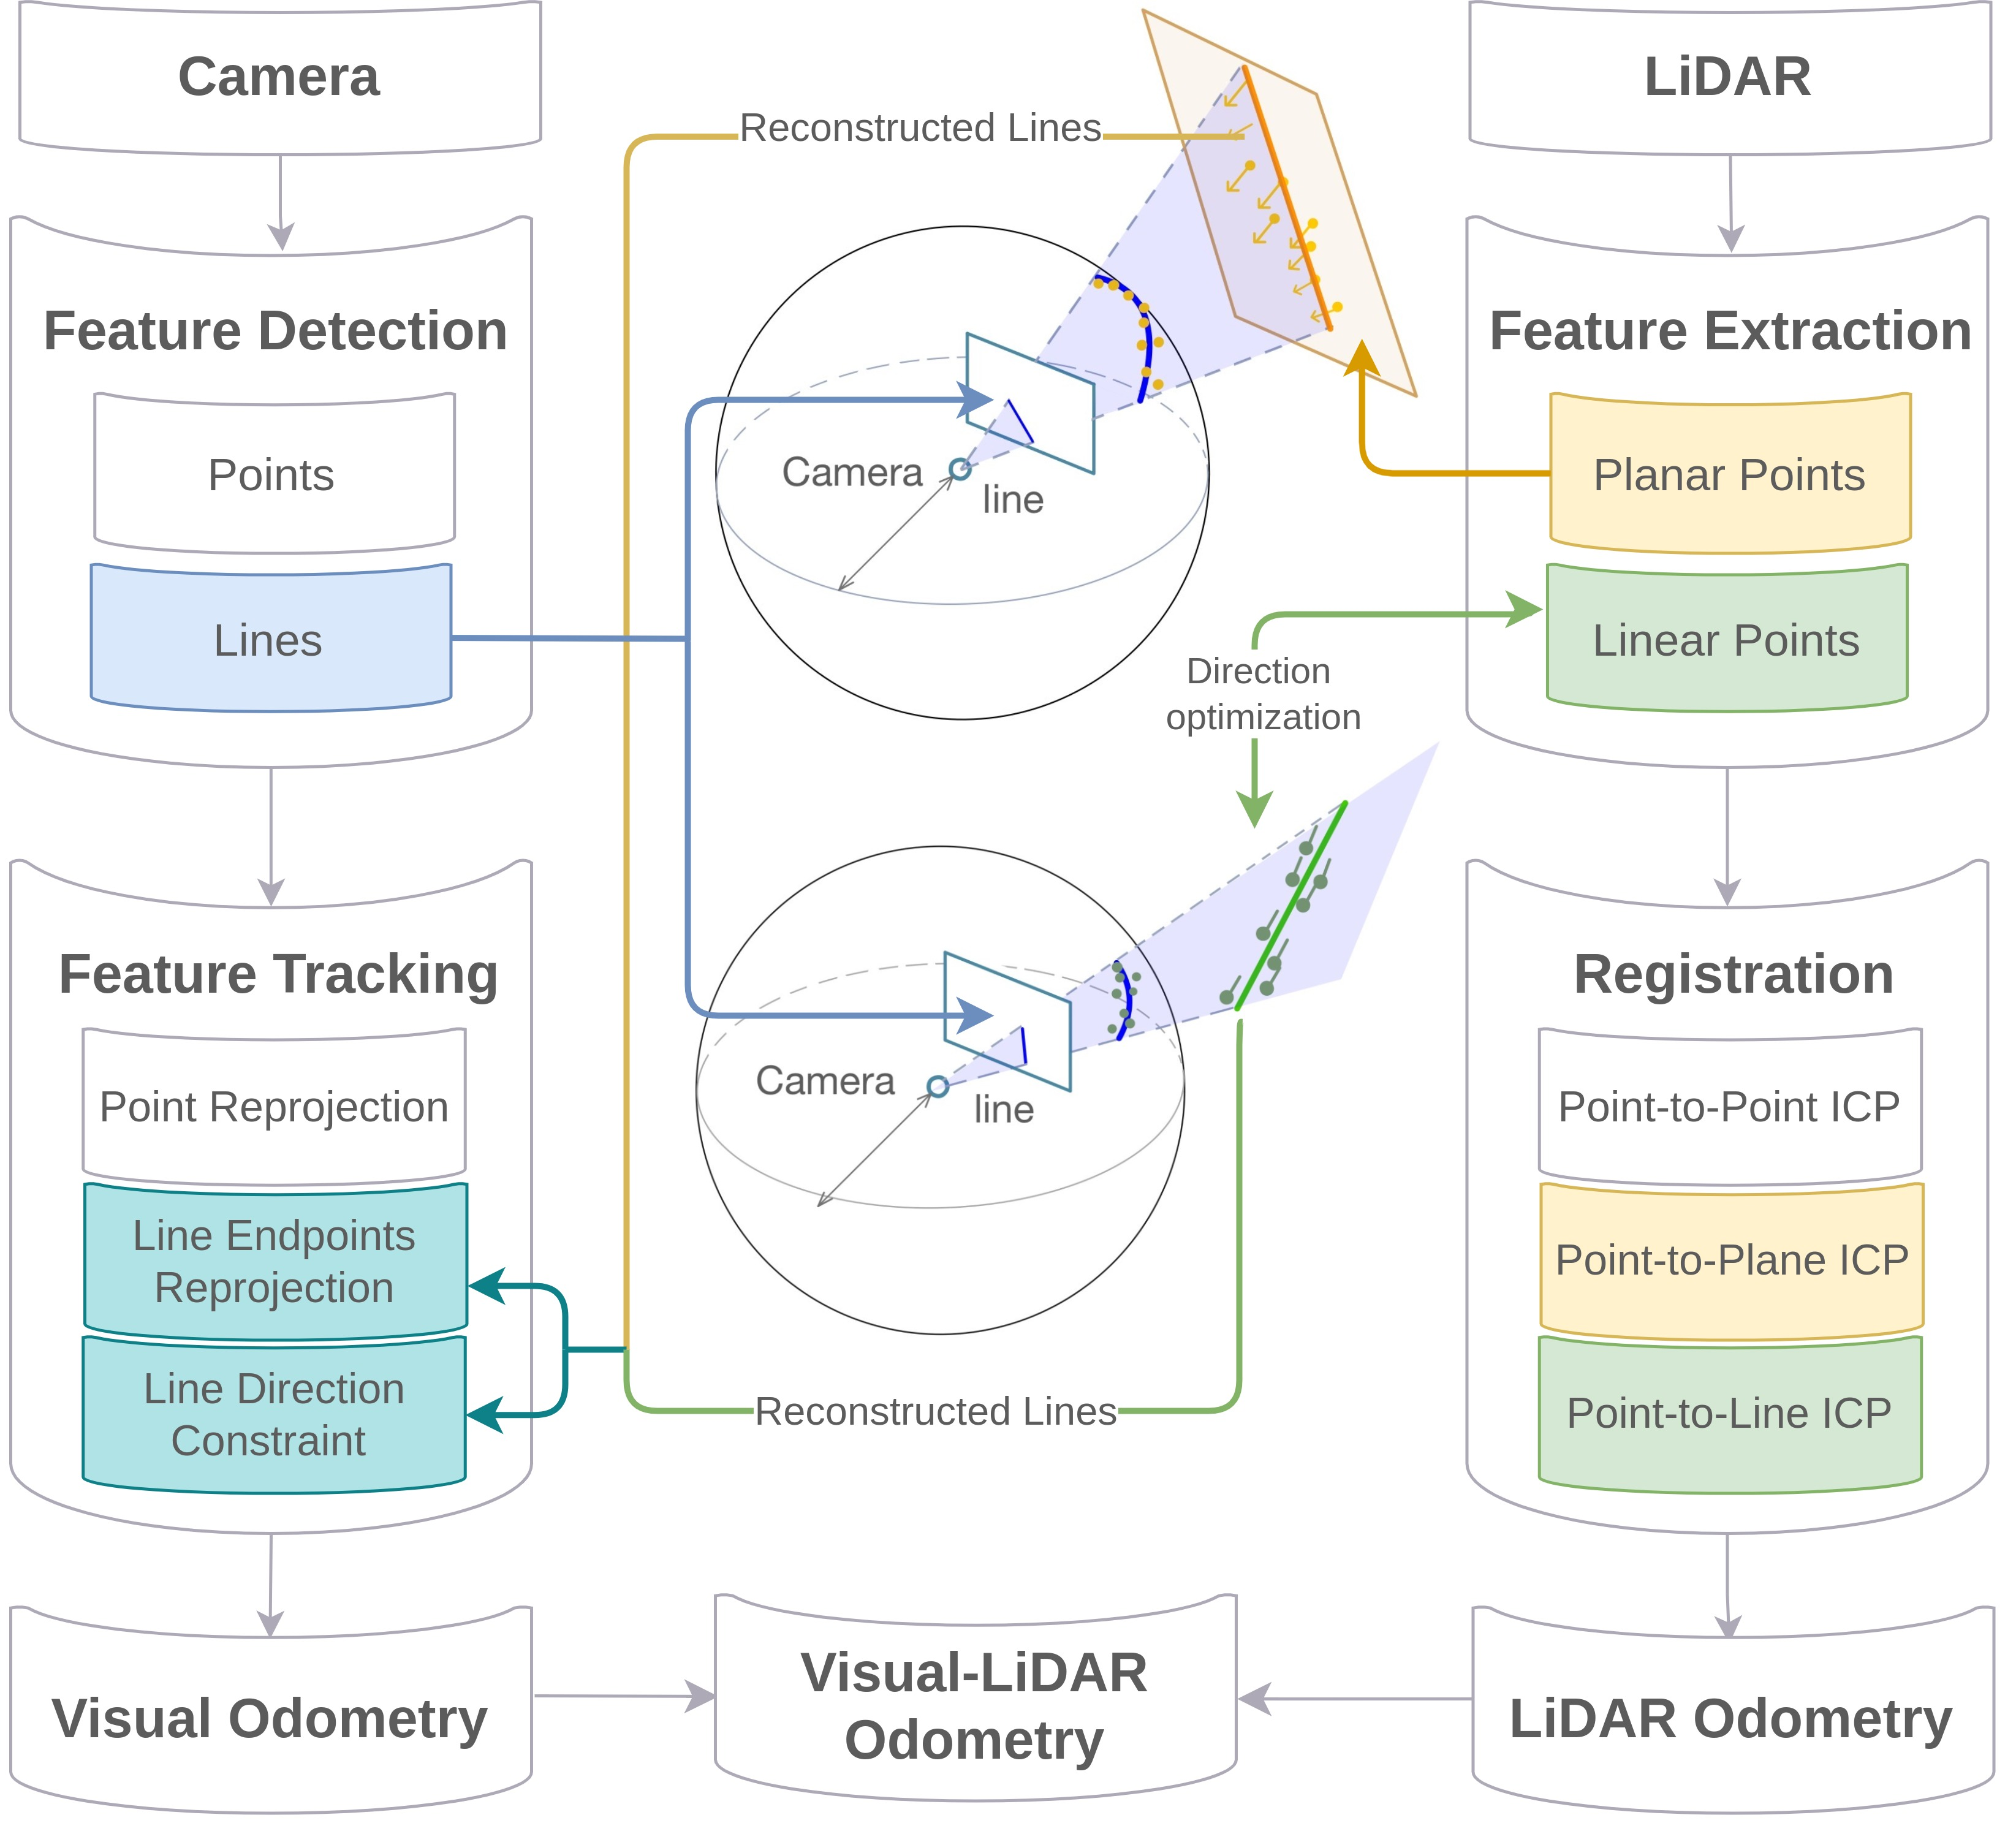
\includegraphics[width=0.62\textwidth]{images/overview.jpg}
  \caption{Overview of our multi-modal SLAM system. It consists of a fusion framework (middle section) and dual systems - the visual SLAM subsystem (left flow) and the LiDAR SLAM subsystem (right flow). The geometric features are extracted by subsystems and then passed to the fusion framework to perform the fusion computations. The generated lines are returned to the subsystems to optimize their odometry and map.} 
  \label{fig:overview}
  \vskip -3ex
\end{figure*}

\noindent\textbf{Multi-modal SLAM.}
Previous multi-modal works can be classified by the type of sensors.
Visual SLAM~\cite{campos2021orb, leutenegger2015keyframe, mur2017visual} optimizes the reprojection error and temporal error by adding other information from IMU and correcting the scales.
Filter-based algorithms~\cite{chen2018review, geneva2020openvins, mourikis2007multi} use inertial measurements for state propagation and update the visual data to improve accuracy.

In the field of high-cost and high-complexity visual-LiDAR-inertial SLAM systems, the optimization-based algorithm LVI-SAM~\cite{shan2021lvi}, consisting of two subsystems, builds on a factor graph and accomplishes tightly-coupled odometry.
TVL-SLAM~\cite{chou2021efficient} proposes a novel large-scale bundle adjustment optimization, which compresses the LiDAR and visual residuals to achieve real-time performance in the degraded environment.
Extended Kalman Filter (EKF) based algorithms~\cite{lin2022r,lin2021r,zuo2019lic,zuo2020lic} contribute to enhancing robustness in environments with weak texture or even no features.

The visual-LiDAR SLAM systems~\cite{seo2019tight, shin2020dvl, zhang2015visual} provide a low-cost, low-compute, high-precision method for mapping and calculating odometry.
DEMO~\cite{zhang2014real, zhang2017real} is the first to associate LiDAR depth measurements with Harris corner features.
However, due to the lack of loop closure, the accumulated residuals cannot be optimized and eliminated.
Liang~\etal~\cite{liang2016visual} address this issue by proposing a scan-matching method with a visual loop detection scheme using ORB features~\cite{rublee2011orb} and a Bag-of-Words model. 

However, the extracted point-only depth as prior factors has a flaw: The multi-sensor aligned error caused by mechanical changes cannot be mitigated without an automatic extrinsic calibration procedure.
LIMO~\cite{graeter2018limo} projects the point cloud onto the image and estimates the point depth by a subset of points within a fixed rectangular region around it. To minimize the number of outliers, a filtering mechanism was introduced. This mechanism limits the depth estimation to subsets within planes.
Huang~\etal~\cite{huang2020LiDAR} explore prior structural information for point-line Bundle Adjustment (BA) and create a novel scale correction scheme.
Although it reduces the system's sensitivity to noise and motion blur, LiDAR-enhanced visual odometry becomes more challenging in underexposed scenarios.
Differing from existing works, our approach is unique in that we incorporate LiDAR-enhanced visual odometry while also developing visual-enhanced LiDAR odometry. This method is designed to be more robust in undesirable lighting conditions.

\noindent\textbf{Line-based SLAM.}
Line-based SLAM performs robustly in man-made scenes, especially when point features are sparse or unevenly distributed in images.
Its map exhibits remarkable richness, comprising a diverse range of geometric elements. Therefore, feature-based and direct visual SLAM systems incorporate geometric features to enhance localization accuracy and robustness in scenes with weak textures and lighting variations.
Visual SLAM~\cite{ram2021rp,  shu2022structure, zhang2020plane}, incorporating plane features, increases the computational complexity of feature extraction and matching.

Feature-based methods~\cite{gee2006real, gomez2019pl, pumarola2017pl, smith2006real} use traditional line detection algorithms like LSD~\cite{engel2014lsd} and perform descriptor-based tracking by minimizing the line projection.
Since the line has only four Degrees of Freedom (DoF), the two-endpoints representation line introduces six parameters, resulting in overparameterization.
Bartoli and Adrien~\cite{bartoli2005structure} propose an orthogonal representation that uses a three-DoF rotation matrix and a one-DoF rotation matrix to update line parameters during optimization.

Lines determined by two-view triangulation often occur during subsequent tracking, which wastes computational resources for detecting, describing, and matching line features.
Problems like line degeneracy occur more frequently when it is close to the epipole.
Lee~\etal~\cite{lee2019elaborate} suggests reconstructing the line segments with multiple views instead of just two.
Furthermore, several algorithms~\cite{lim2021avoiding, yang2019visual} investigate different scenarios of degenerate motion.
They modify LSD and set additional parameters to extract discernable long-line features to prevent this degeneration.

Many visual SLAMs~\cite{georgis2022vp, lee2021plf, lim2022uv, wang2021vanishing} extract vanishing points to add constraints associated with parallel 3D lines to optimize robot pose estimation.
In addition, the PLF-VINS algorithm~\cite{lee2021plf} also integrates point-line coupling residuals based on the similarity of corner points and line features.
This integration ensures accurate depth estimation.

Line-based visual SLAM is commonly used in man-made indoor scenes. Unlike existing works, our approach stands out by combining the accurate geometric features of a LiDAR point cloud with the overall structural information from an image. This results in more effective utilization of line features in a wider range of scenarios.


